\documentclass{article}

\usepackage{xeCJK}
\usepackage[utf8]{inputenc}
\usepackage[a4paper, hmargin={2.8cm, 2.8cm}, vmargin={2.5cm, 2.5cm}]{geometry}
\usepackage{amsmath,amssymb,amsthm} %Matematik symboler og mulighed for "sætninger"
\usepackage{indentfirst}
\usepackage{tikz}

\begin{document}

\section{}

\begin{enumerate}

\item 已知$a$,$b$为两个连续的整数,且$a<\sqrt{28}<b$. 则$a+b=$?
\vspace{15em}

\item 计算:$\sqrt{8}-\sqrt{2}$.
\vspace{15em}

\item 当$x=\sqrt{2}$时,$\dfrac{x^2-1}{x^2-x}-1=$?
\vspace{15em}

\item 使$\sqrt{4x-1}$有意义的$x$的取值范围是
\vspace{15em}

\item 设$a=\sqrt{19}-1$. $a$在两个相邻整数之间. 则这两个数是?
\vspace{15em}

\item 实数$a$在数轴上的位置如图所示. 则$\sqrt{(a-4)^2}+\sqrt{(a-11)^2}$化简之后的值是?
\\ \vspace{1em}

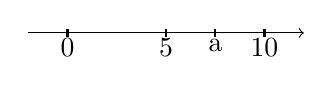
\begin{tikzpicture}[scale=0.25] % Scales the entire image
	% Draw the number line
	\draw[->] (-2,0) -- (12,0); % Axis with arrow
	\foreach \x in {0,5,10} % Draw ticks at 0, 5, and 10
	\draw[shift={(\x,0)}, thick] (0,-6pt) -- (0,6pt) node[below] {\x};
	
	% Mark the point "a" between 5 and 10
	\draw[shift={(7.5,0)}, thick] (0,-6pt) -- (0,6pt) node[below] {a};
\end{tikzpicture}
\vspace{15em}

\item 若$\sqrt{x+y-1}+(y+3)^2=0$, 则$x-y$的值是? 
\vspace{15em}

\item 若$\sqrt{(2a-1)^2}=1-2a$, 则

\noindent
$\mathbf{A}$: $a < \frac{1}{2}$ \hspace{1cm}
$\mathbf{B}$: $a \leqslant \frac{1}{2}$ \hspace{1cm}
$\mathbf{C}$: $a > \frac{1}{2}$ \hspace{1cm}
$\mathbf{D}$: $a \geqslant \frac{1}{2}$
\vspace{15em}

\item 已知$a=\sqrt{2}+1$. 求$\left(\dfrac{2a}{a-1}+\dfrac{a}{1-a}\right)\cdot\dfrac{1}{a}$.
\vspace{15em}

\item 已知$a=\sqrt{2}-1$. 计算$\left( a - 1 + \dfrac{2}{a+1}\right)\cdot\dfrac{1}{a^2+1}$.
\vspace{15em}

\item 解方程 $\begin{cases}
3x+6y=10\\
6x+3y=8
\end{cases}$. 并求$\sqrt{xy}$的值.
\vspace{15em}

\item 已知$x=\dfrac{\sqrt{3}}{2}$. 求$\left(\dfrac{3x}{x+1}-\dfrac{x}{x-1}\right)\cdot\dfrac{x^2-1}{x-2}$.
\end{enumerate}
\end{document}